%%%%%%%%%%%%%%%%%%%%%%%%%%%%%%%%%%%%%%%%%
% Beamer Presentation
% LaTeX Template
% Version 1.0 (10/11/12)
%
% This template has been downloaded from:
% http://www.LaTeXTemplates.com
%
% License:
% CC BY-NC-SA 3.0 (http://creativecommons.org/licenses/by-nc-sa/3.0/)
%
%%%%%%%%%%%%%%%%%%%%%%%%%%%%%%%%%%%%%%%%%

%----------------------------------------------------------------------------------------
%	PACKAGES AND THEMES
%----------------------------------------------------------------------------------------

\documentclass{beamer}

\mode<presentation> {
\usetheme{Madrid}
}

\usepackage{graphicx} % Allows including images
\usepackage{booktabs} % Allows the use of \toprule, \midrule and \bottomrule in tables

%----------------------------------------------------------------------------------------
%	TITLE PAGE
%----------------------------------------------------------------------------------------

\title[Drought Resiliency]{What Makes Communities Resilient to Drought?} 

\author[DS421]{Dan Blaustein-Rejito \inst{1} \and Ian Bolliger \inst{2} \and Hal Gordon \inst{3} \and Andy Hultgren \inst{3} \and Yang Ju \inst{4} \and Kate Pennington \inst{3} \and Sara Stoudt \inst{5}}
\institute[UC Berkeley] 
{
University of California, Berkeley: DS421 \\
\medskip
\inst{1} GSPP \and \inst{2} ERG \and \inst{3} ARE \and \inst{4} LAEP \and \inst{5} Stats\\ 
\medskip
\textit{danr@berkeley.edu \and bolliger@berkeley.edu \and halgordon@berkeley.edu \and hultgren@berkeley.edu \and yangju90@berkeley.edu \and kate.pennington@berkeley.edu \and sstoudt@berkeley.edu} 
}
\date{\today}

\makeatletter
\def\beamer@andinst{\quad}
\makeatother

\begin{document}

\begin{frame}
\titlepage 
\end{frame}

\begin{frame}
\frametitle{Overview}
\tableofcontents
\end{frame}

%----------------------------------------------------------------------------------------
%	PRESENTATION SLIDES
%----------------------------------------------------------------------------------------

%------------------------------------------------
\section{Introduction}
%------------------------------------------------

\begin{frame}
	\frametitle{Drought}
	\begin{itemize} \itemsep1em
		\item In April 2016 in the United States: 
			\begin{itemize}
				\item 14\% of land was in drought and 34\% was abnormally dry.
				\item 84.3 million people live in drought-affected areas, and 17.5 million live in areas experiencing ”exceptional drought”
			\end{itemize}
		\item In California:
			\begin{itemize}
				\item 90\% of the state is in drought and more than 50\% is in severe to exceptional drought.
				\item 84.3 million people live in drought-affected areas, and 17.5 million live in areas experiencing ”exceptional drought”
			\end{itemize} 
	\end{itemize}
\end{frame}

\begin{frame}
\frametitle{Drought, April 19, 2016}
	\begin{figure}
		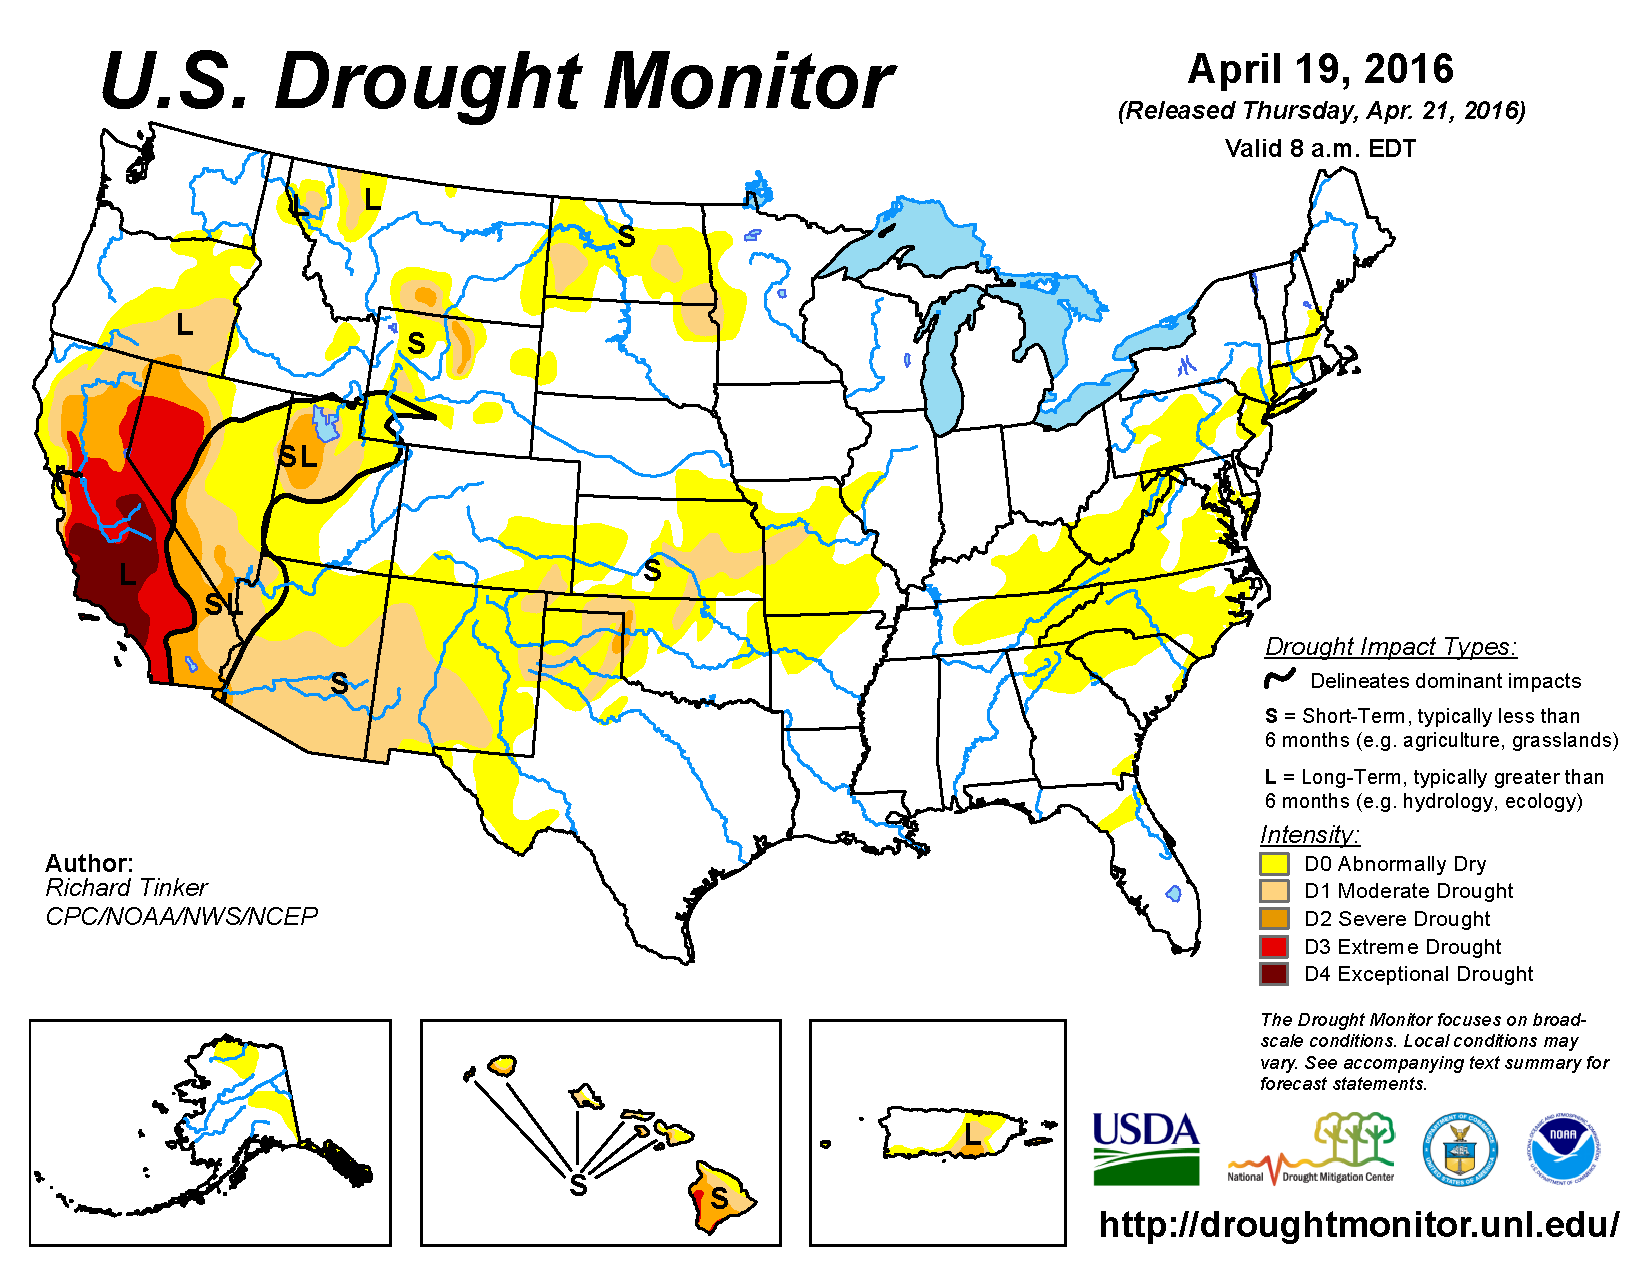
\includegraphics[width=0.8\linewidth]{20160419_usdm}
	\end{figure}	
\end{frame}

\begin{frame}
	\frametitle{Drought}
	\begin{itemize} \itemsep1em
		\item Climate change is likely to increase the length and severity
		\item Drought will effect all regions and populations at one time or another
		\item Resilience, not just risk of drought, will have far reaching implications for welfare changes from climate change.
	\end{itemize}	
\end{frame}

%------------------------------------------------
\section{Model}
%------------------------------------------------
\subsection{First Stage}

\begin{frame}
	\frametitle{Model}
	\textbf{First Stage Equation}
	\begin{equation}
		y_{i,t} = \beta_{i} D_{i,t} + \alpha_i + \tau_i t + \gamma_{s,t} + \epsilon_{i,t}
	\end{equation}
	Where:
	\begin{itemize}
		\item $D_{i,t}$ refers to the number of days in U.S. Drought Survey bins 2-4 in county $i$ and year $t$
		\item $\alpha_i$ are county fixed effects controlling for time-invariant differences between counties
		\item $\tau_i$ is the coefficient on a county level linear time trend
		\item $\gamma_{s,t}$ are state-by-year fixed effects controlling for state level time trends common across all counties $i \in s$
	\end{itemize}
\end{frame}

\begin{frame}
	\frametitle{Model Details}
	\textbf{First Stage Equation}
	\begin{itemize}  \itemsep1em
		\item The state-by-year fixed effects will non-parametrically account for national trends in the outcome of interest as well as state-level trends
		\item The identifying variation in this model is within-county, annual deviations from the county time trend and from statewide annual average drought levels
		\item Standard errors will need to be corrected for serial correlation over space and time
	\end{itemize}
\end{frame}


%------------------------------------------------
\subsection{Second Stage}

\begin{frame}
	\frametitle{Model}
	\textbf{Second Stage Equation}
	\begin{equation}
		\beta_i = \rho_0 + \boldsymbol{\delta} \mathbf{X}_i + \nu_i
	\end{equation}
	Where:
	\begin{itemize}
		\item $\beta_i$ come from Eq.(1) for a given outcome
		\item $\mathbf{X}_i$ represents a vector of county characteristics such as urban/rural, proportion below age 5 or above age 65, home ownership, median cost of residential water bill
		\item $\boldsymbol{\delta}$ is a vector of the associated coefficients for state level time trends common across all counties $i \in s$
	\end{itemize}
\end{frame}


\begin{frame}
	\frametitle{Model Details}
	\textbf{Second Stage Equation}
	\begin{itemize}  \itemsep1em
		\item This regression is cross-sectional and therefore not well identified from a causal perspective
		\item Model will illustrate how "drought resilience" (a low value of $\beta_i$) covaries with a set of common county socioeconomic characteristics
		\item We correct OLS standard errors by clustering over space
	\end{itemize}
\end{frame}

%------------------------------------------------
\section{DATA}
%------------------------------------------------

\begin{frame}
	\frametitle{Stage 1 Data: 2005-2014}
		\begin{equation*}
			y_{i,t} = \beta_{i} D_{i,t} + \alpha_i + \tau_i t + \gamma_{s,t} + \epsilon_{i,t}
		\end{equation*}
	\textbf{Left Hand Side}
	\begin{itemize}  \itemsep1em
		\item \textbf{US Drought Monitor:}
		\begin{itemize}
			\item Scale from 0-4 updated weekly
			\item we create a 1-year, 3-year, and 5-year measure
		\end{itemize}
	\end{itemize}
	\textbf{Right Hand Side}
	\begin{itemize}
		\item \textbf{Mortality:}
		\begin{itemize}
			\item Annual CDC WONDER database
			\item Over-65 and all-ages
		\end{itemize} 
		\item \textbf{Yields:}
		\begin{itemize}
			\item Annual USDA crop yield
			\item Corn, soybeans, and wheat
		\end{itemize}
		\item \textbf{Employment:}
		\begin{itemize}
			\item United States Bureau of Labor Statistics
		\end{itemize}
	\end{itemize}
\end{frame}

\begin{frame}
	\frametitle{Stage 2 Data}
	\begin{equation*}
	\beta_i = \rho_0 + \boldsymbol{\delta} \mathbf{X}_i + \nu_i
	\end{equation*}
	\textbf{Left Hand Side}
	\begin{itemize} 
		\item $\hat{\beta}$ from the first stage.
	\end{itemize}
	\textbf{Right Hand Side}
	\begin{itemize}
		\item \textbf{American Community Survey:}
		\begin{itemize}
			\item Annual (2005-2014) survey conducted by US Census
			\item Over 65, Under 5, Race, Ethnicity, Sex, Work in farming or ranching, Household Income, Household water bills
		\end{itemize} 
		\item \textbf{Water Usage:}
		\begin{itemize}
			\item EPA Facility Registry Service
			\item Count of facilities from high water use industries (agriculture, manufacturing and energy) per county
		\end{itemize}
	\end{itemize}
\end{frame}

\begin{frame}
\frametitle{Blocks of Highlighted Text}
\begin{block}{Block 1}
Lorem ipsum dolor sit amet, consectetur adipiscing elit. Integer lectus nisl, ultricies in feugiat rutrum, porttitor sit amet augue. Aliquam ut tortor mauris. Sed volutpat ante purus, quis accumsan dolor.
\end{block}

\begin{block}{Block 2}
Pellentesque sed tellus purus. Class aptent taciti sociosqu ad litora torquent per conubia nostra, per inceptos himenaeos. Vestibulum quis magna at risus dictum tempor eu vitae velit.
\end{block}

\begin{block}{Block 3}
Suspendisse tincidunt sagittis gravida. Curabitur condimentum, enim sed venenatis rutrum, ipsum neque consectetur orci, sed blandit justo nisi ac lacus.
\end{block}
\end{frame}

%------------------------------------------------

\begin{frame}
\frametitle{Multiple Columns}
\begin{columns}[c] % The "c" option specifies centered vertical alignment while the "t" option is used for top vertical alignment

\column{.45\textwidth} % Left column and width
\textbf{Heading}
\begin{enumerate}
\item Statement
\item Explanation
\item Example
\end{enumerate}

\column{.5\textwidth} % Right column and width
Lorem ipsum dolor sit amet, consectetur adipiscing elit. Integer lectus nisl, ultricies in feugiat rutrum, porttitor sit amet augue. Aliquam ut tortor mauris. Solutpat ante purus, quis accumsan dolor.

\end{columns}
\end{frame}


\begin{frame}
\frametitle{Table}
\begin{table}
\begin{tabular}{l l l}
\toprule
\textbf{Treatments} & \textbf{Response 1} & \textbf{Response 2}\\
\midrule
Treatment 1 & 0.0003262 & 0.562 \\
Treatment 2 & 0.0015681 & 0.910 \\
Treatment 3 & 0.0009271 & 0.296 \\
\bottomrule
\end{tabular}
\caption{Table caption}
\end{table}
\end{frame}

%------------------------------------------------

\begin{frame}
\frametitle{Theorem}
\begin{theorem}[Mass--energy equivalence]
$E = mc^2$
\end{theorem}
\end{frame}

%------------------------------------------------

\begin{frame}[fragile] % Need to use the fragile option when verbatim is used in the slide
\frametitle{Verbatim}
\begin{example}[Theorem Slide Code]
\begin{verbatim}
\begin{frame}
\frametitle{Theorem}
\begin{theorem}[Mass--energy equivalence]
$E = mc^2$
\end{theorem}
\end{frame}\end{verbatim}
\end{example}
\end{frame}

%------------------------------------------------

\begin{frame}
\frametitle{Figure}
Uncomment the code on this slide to include your own image from the same directory as the template .TeX file.
%\begin{figure}
%\includegraphics[width=0.8\linewidth]{test}
%\end{figure}
\end{frame}

%------------------------------------------------

\begin{frame}[fragile] % Need to use the fragile option when verbatim is used in the slide
\frametitle{Citation}
An example of the \verb|\cite| command to cite within the presentation:\\~

This statement requires citation \cite{p1}.
\end{frame}

%------------------------------------------------

\begin{frame}
\frametitle{References}
\footnotesize{
\begin{thebibliography}{99} % Beamer does not support BibTeX so references must be inserted manually as below
\bibitem[Smith, 2012]{p1} John Smith (2012)
\newblock Title of the publication
\newblock \emph{Journal Name} 12(3), 45 -- 678.
\end{thebibliography}
}
\end{frame}

%------------------------------------------------

\begin{frame}
\Huge{\centerline{The End}}
\end{frame}

%----------------------------------------------------------------------------------------

\end{document} 